\subsection{Messung der Brennweite über die Linsengleichung}
Die Messwerte der Gegenstandsweite $g$ und der Bildweite $b$ zu beiden verwendeten Linsen sind in Tabelle \ref{tab:brennweite} notiert.
Die Brennweiten werden mithilfe von Gleichung \eqref{eqn:linse} berechnet.
\begin{table}[h!]
  \centering
  \caption{Messdaten zu den Brennweiten $f_{\text{1, theo}}=\SI{0.1}{m}$ und $f_{\text{2, theo}}=\SI{0.05}{m}$}
  \label{tab:brennweite}
  \begin{tabular}{c c c c c c}
    \toprule
    \multicolumn{3}{c}{$f_{\text{1, theo}}=\SI{0.1}{m}$} & \multicolumn{3}{c}{$f_{\text{2, theo}}=\SI{0.05}{m}$}\\
      g/m     &   b/m     &   $f_{1}$/m   &   g/m     &   b/m   &   $f_{2}$/m\\
      \midrule
      0,15    &   0,294   &   0,0993    &   0,08    &   0,136   &   0,0504  \\
      0,12    &   0,620   &   0,1005    &   0,10    &   0,095   &   0,0487  \\
      0,18    &   0,224   &   0,0998    &   0,12    &   0,085   &   0,0498  \\
      0,20    &   0,195   &   0,0987    &   0,13    &   0,083   &   0,0507  \\
      0,22    &   0,180   &   0,0990    &   0,15    &   0,076   &   0,0504  \\
      0,25    &   0,163   &   0,0987    &   0,18    &   0,070   &   0,0504  \\
      0,28    &   0,153   &   0,0989    &   0,20    &   0,068   &   0,0508  \\
      0,30    &   0,145   &   0,0978    &   0,22    &   0,066   &   0,0508  \\
      0,32    &   0,142   &   0,0984    &   0,25    &   0,062   &   0,0497  \\
      0,35    &   0,137   &   0,0985    &   \\

    \bottomrule
  \end{tabular}
\end{table}

%\end{landscape}
%\end{document}

Der Mittelwert $\mu$ berechnet sich allgemein über
\begin{align}
  \overline{x}= \frac{1}{N} \sum_{n=1}^{N} x_{n}.
  \label{eqn:mu}
\end{align}
Der Fehler, der durch das Mitteln gemacht wird, entspricht der Standardabweichung $\sigma$:
\begin{align}
  \sigma= \sqrt{ \frac{1}{N-1} \sum_{n=1}^{N} ( x_{n} - \overline{x})^2}.
  \label{eqn:std}
\end{align}
Die gemittelten Brennweiten ergeben sich dann zu:
\begin{align*}
  \overline{f_{1}} &=& \SI{0.09896 \pm 0.00076}{m}\\
  \overline{f_{2}} &=& \SI{0.05019 \pm 0.00069}{m}.\\
\end{align*}
Desweiteren werden die Werte der Bildweite $b$ gegen die Gegenstandsweiten $g$ aufgetragen (Abb. \ref{fig:f100}, \ref{fig:f50}).
Die Wertepaare werden durch eine Gerade verbunden um die Messgenauigkeit graphisch darzustellen.
\begin{figure}[h!]
  \centering
  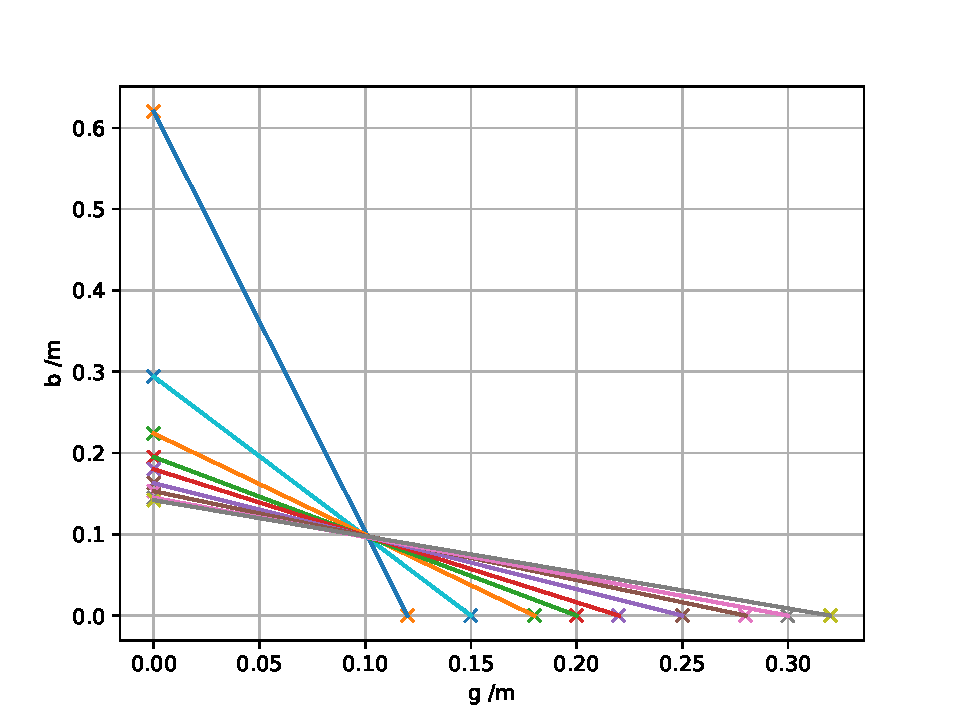
\includegraphics[width=\textwidth]{f100.pdf}
  \caption{Darstellung der Messgenauigkeit für $f_{\text{1, theo}}=\SI{0.1}{m}$}
  \label{fig:f100}
\end{figure}
\begin{figure}[h!]
  \centering
  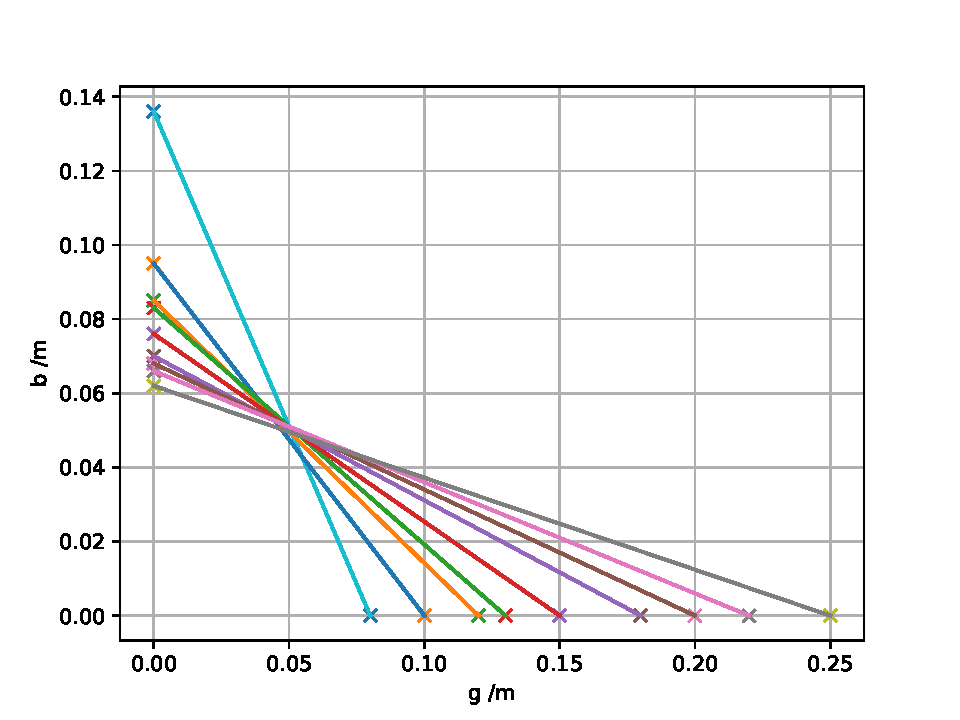
\includegraphics[width=\textwidth]{f50.pdf}
  \caption{Darstellung der Messgenauigkeit für $f_{\text{2, theo}}=\SI{0.05}{m}$}
  \label{fig:f50}
\end{figure}
In beiden Abbildungen entspricht jeweils $g$- und $b$-Koordinate des Schnittpunkts aller Geraden der Brennweite.
So liegt in Abbildung \ref{fig:f100} der Schnittpunkt etwa bei $g=b=\SI{0.1}{m}$, was zu der Brennweite $f_{\text{1, theo}}=\SI{0.1}{m}$ passt.
In Abbildung \ref{fig:f50} liegt der Schnittpunkt bei $g=b=\SI{0.05}{m}$.
Diese Werte entsprechen ebenfalls zu der angegebenen Brennweite $f_{\text{2, theo}}=\SI{0.05}{m}$ der Linse.
\FloatBarrier

\subsection{Messung der Brennweite nach Bessel}
\label{kap:bessel}
Die gemessenen Brennweiten und Gegenstandsweiten sind in Tabelle \ref{tab:bessel} notiert.
\begin{table}[h!]
  \centering
  \caption{Messdaten zu den Gegenstandsweiten $g_{1}$ und $g_{2}$ und den Bildweiten $b_{1}$ und $b_{2}$ bei einer Linse mit $f_{\text{theo}}=\SI{0.1}{m}$}
  \label{tab:bessel}
  \begin{tabular}{c c c c c c c c c c}
    \toprule
%    \multicolumn{3}{c}{$f_{\text{1, theo}}=\SI{0.1}{m}$} & \multicolumn{3}{c}{$f_{\text{2, theo}}=\SI{0.05}{m}$}\\
      $g_{1}$/m & $b_{1}$/m  &   $g_{2}$/m     &   $b_{2}$/m   &   $e$   &   $d_{1}$    &  $d_{2}$  &  $d$  &   $f$/m\\
      \midrule
       0,678  &  0,122   &   0,115    &   0,685    &  0,800   &  0,570  &   0,556   &  0,563 \pm 0,010   &  0,101 \pm 0,004  \\
       0,735  &  0,115   &   0,121    &   0,729    &  0,850   &  0,608  &   0,620   &  0,614 \pm 0,009   &  0,102 \pm 0,003  \\
       0,788  &  0,112   &   0,118    &   0,782    &  0,900   &  0,664  &   0,676   &  0,670 \pm 0,009   &  0,100 \pm 0,003  \\
       0,838  &  0,112   &   0,116    &   0,834    &  0,950   &  0,718  &   0,726   &  0,722 \pm 0,006   &  0,100 \pm 0,002  \\
       0,889  &  0,111   &   0,116    &   0,884    &  1,000   &  0,768  &   0,778   &  0,773 \pm 0,007   &  0,101 \pm 0,003  \\
       0,937  &  0,113   &   0,115    &   0,935    &  1,050   &  0,820  &   0,824   &  0,822 \pm 0,003   &  0,102 \pm 0,001  \\
       0,989  &  0,111   &   0,115    &   0,985    &  1,100   &  0,870  &   0,878   &  0,874 \pm 0,006   &  0,101 \pm 0,002  \\
       1,040  &  0,110   &   0,115    &   1,035    &  1,150   &  0,920  &   0,930   &  0,925 \pm 0,007   &  0,102 \pm 0,003  \\
       1,090  &  0,110   &   0,114    &   1,086    &  1,200   &  0,972  &   0,980   &  0,976 \pm 0,006   &  0,102 \pm 0,002  \\
       1,139  &  0,111   &   0,114    &   1,136    &  1,250   &  1,022  &   1,028   &  1,025 \pm 0,004   &  0,102 \pm 0,002  \\

    \bottomrule
  \end{tabular}
\end{table}

%\end{landscape}
%\end{document}

Für die Bestimmung des Abstands $d$ zwischen den Linsen werden die Abstände $d_{1}$ und $d_{2}$ nach Gleichung \eqref{eqn:mu} gemittelt.
Der Fehler der Messung ergibt sich über die Standardabweichung nach Gleichung \eqref{eqn:std}.
Die Brennweite wird über Gleichung \eqref{eqn:bessel} berechnet.
Die Fehler berechnen sich nach der Gauß'schen Fehlerfortpflanzung:
\begin{align*}
  \Delta f_{1}= \sqrt{ \left( \frac{df}{d d} \right)^2 \Delta d^2 }= \sqrt{ \left( -\frac{d}{2e}\right)^2 \Delta d^2}.
\end{align*}
Die einzelnen Brennweiten werden nun nach Gleichung \eqref{eqn:mu} gemittelt und der Fehler über die Standardabweichung nach Gleichung \eqref{eqn:std} ermittelt:
\begin{align*}
  \overline{f_{1}}= \SI{0.1013 \pm 0.0008}{m}.
\end{align*}
\FloatBarrier

\subsection{Untersuchung der chromatischen Abberation}
Die Messdaten zur Untersuchung der chromatischen Abberation sind in Tabelle \ref{tab:chrom} aufgetragen.
\begin{table}[h!]
  \centering
  \caption{Messdaten zur chromatischen Abberation bei einem roten Filter und einem blauen Filter}
  \label{tab:chrom}
  \begin{tabular}{c c c c c c c c c}
    \toprule
    \multicolumn{9}{c}{Blauer Filter}\\
      \midrule
    $g_{1}$/m & $b_{1}$/m & $g_{2}$/m & $b_{2}$/m &   $e$    & $d_{1}$   &  $d_{2}$  &   $d$               &   $f$/m            \\
      \midrule
      0,686   &   0,114   &   0,120   &   0,680   &   0,800  &   0,572   &   0,560   &   0,566 \pm 0,009   &   0,100 \pm 0,003  \\
      0,736   &   0,114   &   0,121   &   0,729   &   0,850  &   0,622   &   0,608   &   0,615 \pm 0,010   &   0,101 \pm 0,004  \\
      0,785   &   0,115   &   0,120   &   0,780   &   0,900  &   0,670   &   0,660   &   0,665 \pm 0,007   &   0,102 \pm 0,003  \\
      0,837   &   0,113   &   0,118   &   0,832   &   0,950  &   0,724   &   0,714   &   0,719 \pm 0,007   &   0,102 \pm 0,003  \\
      0,887   &   0,113   &   0,116   &   0,884   &   1,000  &   0,774   &   0,768   &   0,771 \pm 0,004   &   0,101 \pm 0,002  \\
      \midrule
    \multicolumn{9}{c}{Roter Filter}\\
      \midrule
      0,684   &   0,116   &   0,121   &   0,679   &   0,80   &   0,568   &   0,558   &   0,563 \pm 0,007   &   0,101 \pm 0,003  \\
      0,735   &   0,115   &   0,121   &   0,729   &   0,85   &   0,620   &   0,608   &   0,614 \pm 0,009   &   0,102 \pm 0,003  \\
      0,784   &   0,116   &   0,121   &   0,779   &   0,90   &   0,668   &   0,658   &   0,663 \pm 0,007   &   0,103 \pm 0,003  \\
      0,837   &   0,113   &   0,119   &   0,831   &   0,95   &   0,724   &   0,712   &   0,718 \pm 0,009   &   0,102 \pm 0,003  \\
      0,886   &   0,114   &   0,118   &   0,882   &   1,00   &   0,772   &   0,764   &   0,768 \pm 0,006   &   0,103 \pm 0,002  \\
    \bottomrule
  \end{tabular}
\end{table}

%\end{landscape}
%\end{document}

Die Rechnungen werden analog zu Kapitel \ref{kap:bessel} durchgeführt.
Die Brennweiten $f$ werden nach Gleichung \eqref{eqn:mu} emittelt.
Es ergeben sich die Brennweiten
\begin{align*}
  \overline{f_{\text{blau}}} &=& \SI{0.1012 \pm 0.0008}{m}\\
  \overline{f_{\text{rot}}}  &=& \SI{0.1022 \pm 0.0008}{m}.\\
\end{align*}

\FloatBarrier

\subsection{Messung der Brennweite und Hauptebenen nach Abbe}
Die Messdaten sind in Tabelle \ref{tab:abbe} notiert.
\begin{table}[h!]
  \centering
  \caption{Messdaten zur Brennweite eines Linsensystems mit $f_{\text{1, theo}}=\SI{0.1}{m}$ und $f_{\text{3, theo}}=\SI{-0.1}{m}$ bei der Gegenstandsgröße $G=\SI{0.03}{m}$}
  \label{tab:abbe}
  \begin{tabular}{c c c c c c c c}
    \toprule
%    \multicolumn{3}{c}{$f_{\text{1, theo}}=\SI{0.1}{m}$} & \multicolumn{3}{c}{$f_{\text{2, theo}}=\SI{0.05}{m}$}\\
      g'/m  &  b'/m   &  B/m     &  V      &  $1+\frac{1}{V}$ &  $1+V$  \\
      \midrule
      0,45  &  0,235  &  0,0260  &  0,867  &  2,1534          &  1,867  \\
      0,50  &  0,195  &  0,0200  &  0,667  &  2,4993          &  1,667  \\
      0,55  &  0,175  &  0,0160  &  0,533  &  2,8762          &  1,533  \\
      0,60  &  0,165  &  0,0140  &  0,467  &  3,1413          &  1,467  \\
      0,65  &  0,154  &  0,0120  &  0,400  &  3,5000          &  1,400  \\
      0,70  &  0,146  &  0,0100  &  0,333  &  4,0030          &  1,333  \\
      0,75  &  0,136  &  0,0090  &  0,300  &  4,3333          &  1,300  \\
      0,80  &  0,135  &  0,0085  &  0,283  &  4,5336          &  1,283  \\
      0,85  &  0,131  &  0,0080  &  0,267  &  4,7453          &  1,267  \\
      0,90  &  0,125  &  0,0070  &  0,233  &  5,2918          &  1,233  \\
    \bottomrule
  \end{tabular}
\end{table}

%\end{landscape}
%\end{document}

Der Abbildungsmaßstab $V$ wird nach Gleichung \eqref{eqn:maßstab} errechnet.
\\In Abbildung \ref{fig:abbe1} ist die Gegenstandsweite $g'$ gegen $1+\frac{1}{V}$ aufgetragen.
\begin{figure}[h!]
  \centering
  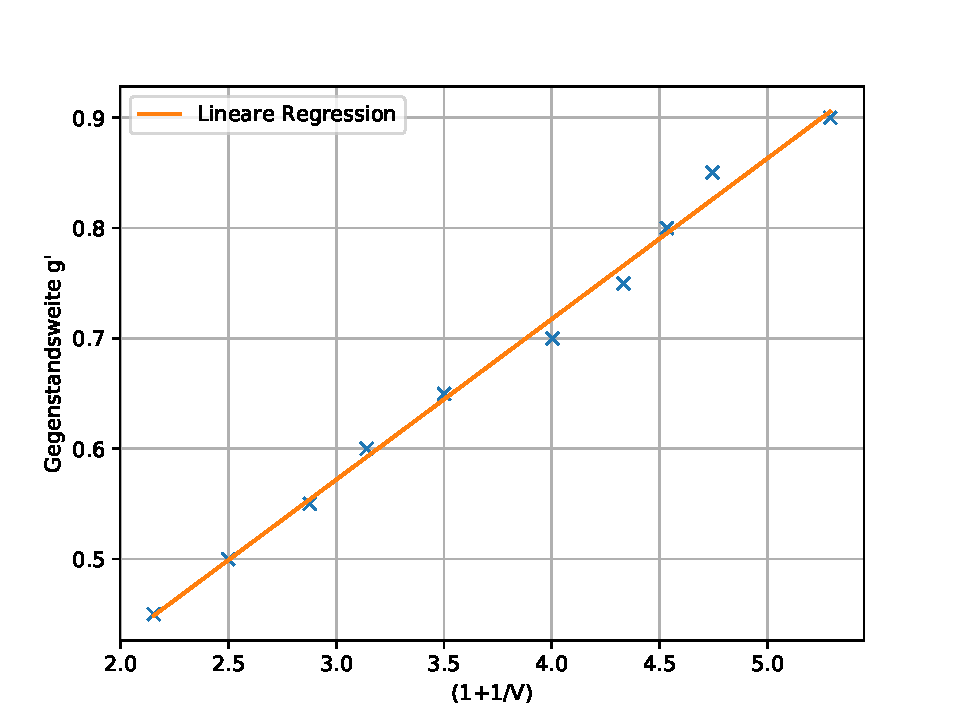
\includegraphics[width=\textwidth]{abbe1.pdf}
  \caption{$g'$ gegen $1+\frac{1}{V}$ zur Bestimmung der Brennweite $f$ und der Hauptebene $h$}
  \label{fig:abbe1}
\end{figure}
Die Gegenstandsweite $g'$ hat einen linearen Zusammenhang zur Brennweite $f$:
\begin{align*}
  g' &=& f && \left(1+\frac{1}{V} \right) && + h && && &&\\
  y  &=& a && x                           && + b.&& && &&\\
\end{align*}
Die lineare Regression der Form mithilfe von Python ergibt die Parameter:
\begin{align*}
  a = f &=& \SI{0.1455 \pm 0.0041}{m}\\
  b = h &=& \SI{0.1355 \pm 0.0158}{m}.\\
\end{align*}
\\Zur Bestimmung der zweiten Hauptebene $h'$ und der Brennweite $f$ wird der lineare Zusammenhang dieser Größen zur Bildweite $b'$ genutzt:
\begin{align*}
  b' &=& f && (1+V) && + h' && && &&\\
  y  &=& c && x     && + d. && && &&\\
\end{align*}
Es wird also $b'$ gegen $1+V$ in Abbildung \ref{fig:abbe2} aufgetragen.
\begin{figure}[h!]
  \centering
  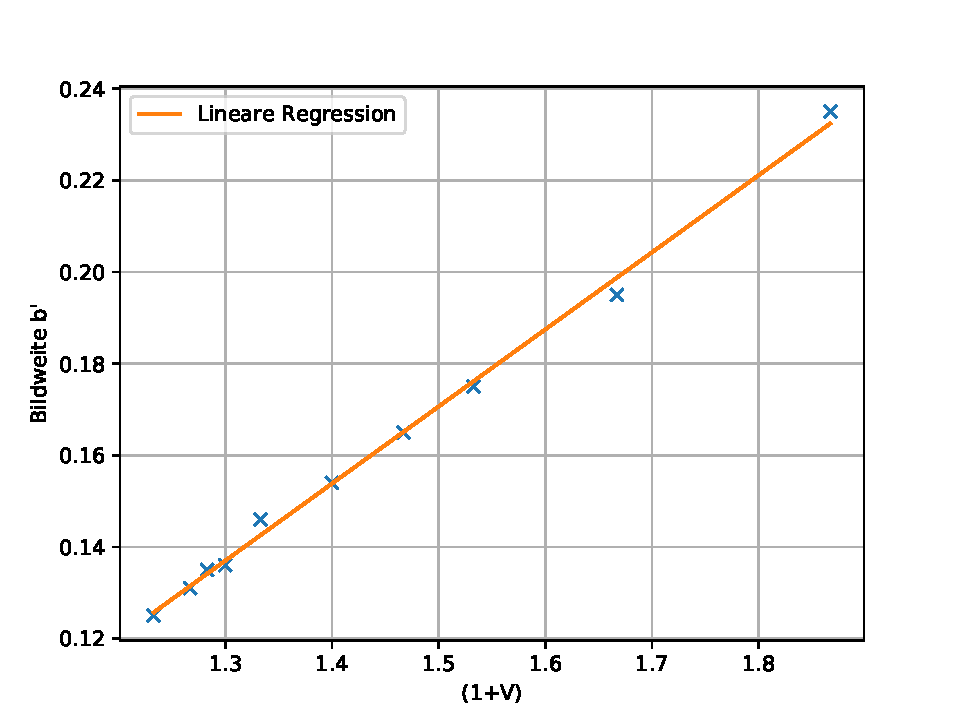
\includegraphics[width=\textwidth]{abbe2.pdf}
  \caption{$b'$ gegen $1+V$ zur Bestimmung der Brennweite $f$ und der Hauptebene $h'$}
  \label{fig:abbe2}
\end{figure}
Es ergeben sich die Parameter
\begin{align*}
  c = f  &=& \SI{ 0.1683 \pm 0.0035}{m}\\
  d = h' &=& \SI{-0.0818 \pm 0.0051}{m}.\\
\end{align*}
Die gemittelte Brennweite beläuft sich zu
\begin{align*}
  \overline{f_{\text{Abbe}}}= \SI{0.1569 \pm 0.0161}{m}.
\end{align*}


\FloatBarrier
